Diffie–Hellman key exchange [\cite{li2010research}] is a method of securely exchanging cryptographic keys over a public channel
and was one of the first public-key protocols
as conceived by Ralph Merkle and named after Whitefield Diffie and Martin Hellman.
DH is one of the earliest practical examples of public key exchange implemented within the field of cryptography.
Published in 1976 by Diffie and Hellman, this is the earliest publicly known work that proposed the idea of a private
key and a corresponding public key.
Traditionally, secure encrypted communication between two parties required that they first exchange keys by some secure physical means,
such as paper key lists transported by a trusted courier.
The Diffie–Hellman key exchange method allows two parties that have no prior knowledge of
each other to jointly establish a shared secret key over an insecure channel.
This key can then be used to encrypt subsequent communications using a symmetric-key cipher.
Although Diffie–Hellman key agreement itself is a non-authenticated key-agreement protocol, it provides the basis for a
variety of authenticated protocols, and is used to provide forward secrecy in Transport Layer Security's ephemeral modes,
referred to as EDH or DHE [\cite{ahirwal2013elliptic}] depending on the cipher suite.

Diffie–Hellman key exchange establishes a shared secret between two parties that can be used for secret communication
for exchanging data over a public network.
An analogy illustrates the concept of public key exchange by using colors instead of very large numbers:
\begin{figure}[H]
    \centering
    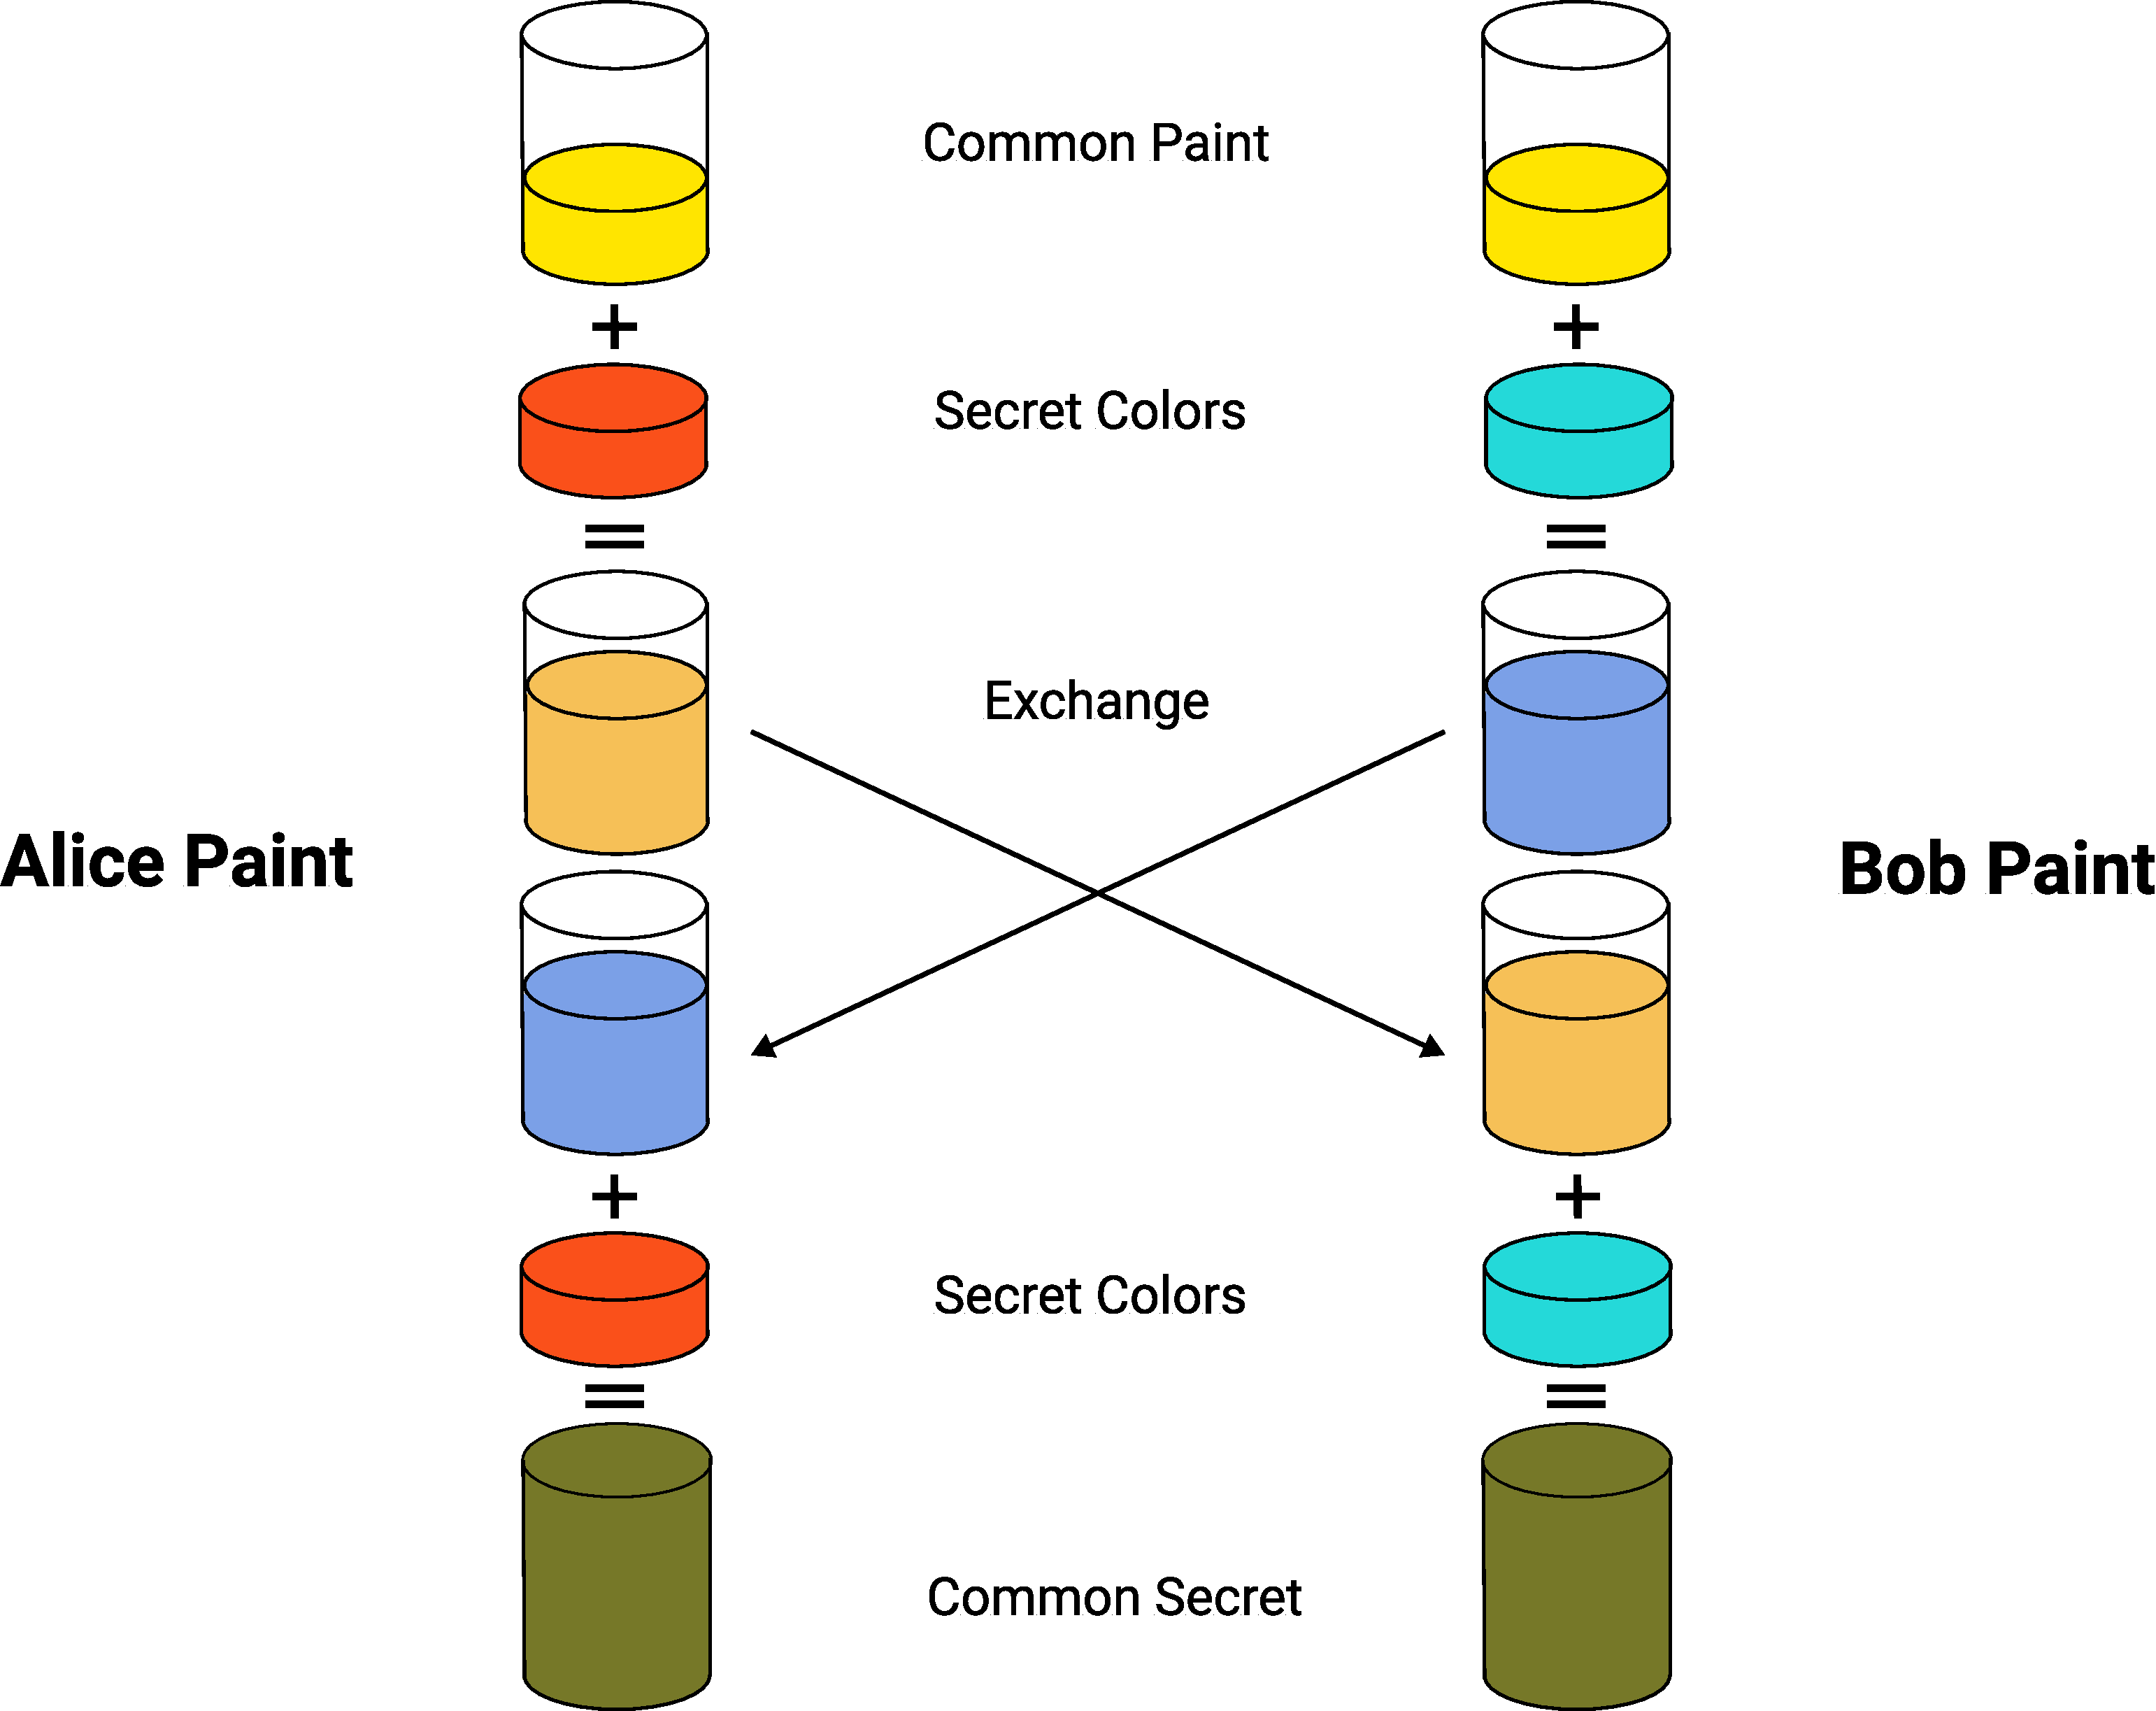
\includegraphics[width=1\textwidth]{Pictures/Diffie-Hellman}
    \caption{Illustration of the concept behind Diffie–Hellman key exchange. Source: }\label{fig:figure4}
\end{figure}
The process begins by having the two parties, Alice and Bob, publicly agree on an arbitrary starting color that does
not need to be kept secret (but should be different every time).
In this example, the color is yellow.
Each person also selects a secret color that they keep to themselves – in this case, red and blue-green.
The crucial part of the process is that Alice and Bob each mix their own secret color together with their mutually
shared color, resulting in orange-tan and light-blue mixtures respectively, and then publicly exchange the two mixed colors.
Finally, each of them mixes the color they received from the partner with their own private color.
The result is a final color mixture (yellow-brown in this case) that is identical to the partner's final color mixture.
If a third party listened to the exchange, it would only know the common color (yellow) and the first mixed colors
(orange-tan and light-blue), but it would be difficult for this party to determine the final secret color (yellow-brown).
Bringing the analogy back to a real-life exchange using large numbers rather than colors, this determination is
computationally expensive.
It is impossible to compute in a practical amount of time even for modern supercomputers.

The simplest and the original implementation of the protocol uses the multiplicative group of integers modulo $P$,
where $P$ is prime, and the generator $G$ which is a primitive root modulo $P$.
These two values are chosen in this way to ensure that the resulting shared secret can take on any value from $1$ to $P-1$.
Here is an example of the protocol
\begin{enumerate}
    \item Given modulus $P$ and generator $G$.
    \item Alice chooses her secret $a$.
    \item Alice sends to Bob $A, \; A = G^a \bmod P$.
    \item Bob chooses his secret $b$.
    \item Bob sends to Alice $B, \; B = G^b \bmod P$.
    \item Alice computes common secret $s, \; s = B^a \bmod P = (G^b \bmod P)^a \bmod P$.
    \item Bob computes common secret $s, \; s = A^b \bmod P = (G^a \bmod P)^b \bmod P$.
    \item Alice and Bob have arrived to the same value
    \[
        A^b \bmod P = G^{ab} \bmod P = G^{ba} \bmod P = B^a \bmod P,
    \]
    more specially,
    \[
        (G^a \bmod P)^b \bmod P = (G^b \bmod P)^a
    \]
\end{enumerate}
However, to reach a satisfactory level of security through DH key exchange a few rules have to be satisfied.
More precisely, Diffie-Hellman works in a multiplicative subgroup of integers modulo a given prime $p$.
To do some DH, you use some DH parameters which are:
\begin{itemize}
    \item p -- a big prime, called the "modulus"
    \item q -- a divisor of $p-1$, called the "subgroup order".
    \item g -- an integer modulo $p$ of order $q$, this means that the smallest integer $k > 0$ such that
    $g^k = 1 \bmod p$ is $k = q$.
\end{itemize}
For DH to be safe, you need the following:

\begin{itemize}
    \item Prime $p$ must defeat attempt at discrete logarithm through Index Calculus.
    This means that $p$ must be large enough, and also must not have any "special structure"
    such as being very close to a power of 2, because such structures allow for improvements in Index Calculus.
    It so happens that size requirements for DH are about the same as the size requirements for RSA,
    though the underlying reason for that is intricate and partly coincidental.
    So, basically, use a random $p$ of 2048 bits, and you will be fine.
    \item Number $q$ should be prime or have a prime divisor whose size is enough to defeat generic algorithms for
    discrete logarithm.
    If the size (in bits) of the largest prime divisor of $q$ is $z$, then generic algorithms have a cost in $2^{z/2}$.
    For best results, arrange for $q$ to be a prime of 256 bits or more.
    \item Systems that use the parameters to perform a DH key exchange must generate a random integer
    between $1$ and $q-1$ uniformly, using a cryptographically strong source of randomness, of course.
    If $q$ is prime and larger than 256 bits, it suffices to choose a 256-bit random value
    to achieve 128-bit of security.
    However, if $q$ is not prime, things are more complex: if $q$ has size $r$ bits,
    and the largest prime divisor of $q$ has size $e$ bits, and $e \geq 256$,
    then one may choose a random value $x$ of size $r-(e-256)$
    bits to get the usual "128-bit security".
    \item When $p$ is a so-called "safe prime", then $p = 2r+1$ for a prime $r$, so for any generator $g$ that is
    not $1$ or $p-1$, the order of $g$ will be either $r$ or $2r$, so it suffices to generate DH secret keys
    $x$ as random 257-bit values.
    The "safe primes" are not actually any safer than other primes,
    except for that point: they tolerate the choice of relatively small DH secret keys for any generator.
    \item Last but not least, DH is a key exchange algorithm that does not,
    inherently, provide authentication or confidentiality.
    DH is "safe" only when used within a protocol that uses DH and other algorithms with proper
    integration to achieve such sought after characteristics as data confidentiality and integrity.
\end{itemize}

Speaking of which, some (many) SSL/TLS implementations did things improperly, in that they
gladly accepted to do DH with weak parameters, in particular a 512-bit modulus.
The protocol itself is suboptimal in its handling of DH because the \texttt{ServerKeyExchange}
message allows the server to send the DH parameters $p$ and $g$ to the client, but not $q$,
leaving the client a bit in the dark.
Thus, the client must either "play safe" and generate its key in the full $1, \;\dots,\; p-1$ range,
or try to use a shorter exponent (say, 256 bits, not 2048) for a reduced computational cost,
but possibly at risk of weakness in case the subgroup order $q$ is not prime.
A better design would have allowed the server to send the value of $q$ and the size of the
biggest prime divisor of $q$.
In that respect, the ECDHE cipher suites of SSL/TLS (DH translated to elliptic curves)
have a better design.

For a practical answer if you are configuring your SSL/TLS server:
you should use a modulus of at least 2048-bit, and a generator $g$ such that the order
of $g$ is a prime $q$ of at least 256 bits;
alternatively, you may use a modulus $p$ which
is a "safe prime", the order of $g$ will then be either a very big prime, or twice
a very big prime, which is almost as good.
Some people feel safer when they generate their DH parameters
"themselves" instead of reusing existing values;
if that's what it takes
to allow you to sleep at night, then do it.

%\subsection{Secrecy Chart}\label{subsec:secrecy-chart}
%The chart below depicts who knows what, again with non-secret values in \textcolor{blue}{blue}, and secret values in \textcolor{red}{red}.
%Here Eve is an eavesdropper – she watches what is sent between Alice and Bob, but she does not alter the contents of their communications.
%\begin{itemize}
%    \item \textcolor{blue}{g} = public (prime) base, known to Alice, Bob, and Eve. $\textcolor{blue}{g = 5}$
%    \item \textcolor{blue}{p} = public (prime) modulus, known to Alice, Bob, and Eve. $\textcolor{blue}{p = 23}$
%    \item \textcolor{red}{a} = Alice's private key, known only to Alice. $\textcolor{red}{a = 6}$
%    \item \textcolor{red}{b} = Bob's private key known only to Bob. $\textcolor{red}{b = 15}$
%    \item \textcolor{blue}{A} = Alice's public key, known to Alice, Bob, and Eve. $\textcolor{blue}{A = g}^{\textcolor{red}{a}} \, mod \, \textcolor{blue}{p = 8}$
%    \item \textcolor{blue}{B} = Bob's public key, known to Alice, Bob, and Eve. $\textcolor{blue}{B = g}^{\textcolor{red}{a}} \, mod \, \textcolor{blue}{p = 8}$
%\end{itemize}
%\begin{center}
%    \begin{table}
%        \begin{tabular}{|c|c|c|c|c|c|}
%            \hline
%            \multicolumn{2}{|c|}{Alice} & \multicolumn{2}{c|}{Bob} & \multicolumn{2}{c|}{Eve}
%            \cr \hline
%            known & unknown & known & unknown & known & unknown
%            \cr \hline
%            $\textcolor{blue}{p = 23}$ & & $\textcolor{blue}{p = 23}$  & & $\textcolor{blue}{p = 23}$ &
%            \cr \hline
%            $\textcolor{blue}{g = 5}$ & & $\textcolor{blue}{g = 5}$ & & $\textcolor{blue}{g = 5}$ &
%            \cr \hline
%            $\textcolor{red}{a = 6}$ & $\textcolor{red}{b}$ & $\textcolor{red}{b = 15}$ & $\textcolor{red}{a}$ & & $\textcolor{red}{a, b}$
%            \cr \hline
%            $\textcolor{blue}{A = 5}^{\textcolor{red}{a}} \, mod \, \textcolor{blue}{23}$ & & $\textcolor{blue}{B = 5}^{\textcolor{red}{b}} \, mod \, \textcolor{blue}{23}$ & & &
%            \cr \hline
%            $\textcolor{blue}{A = 5}^{\textcolor{red}{6}} \, mod \, \textcolor{blue}{23} = \textcolor{blue}{8}$ & & $\textcolor{blue}{B = 5}^{\textcolor{red}{15}} \, mod \, \textcolor{blue}{23} = \textcolor{blue}{19}$ & & &
%            \cr \hline
%            $\textbf{\textcolor{blue}{B}} = \textbf{\textcolor{blue}{19}}$ & & $\textbf{\textcolor{blue}{A}} = \textbf{\textcolor{blue}{8}}$ & & $\textcolor{blue}{A} = \textcolor{blue}{8}$, $\textcolor{blue}{B} = \textcolor{blue}{19}$ &
%            \cr \hline
%            $\textbf{\textcolor{red}{s}} = \textcolor{blue}{B}^{\textcolor{red}{a}} \, mod \, \textcolor{blue}{23}$ & & $\textbf{\textcolor{red}{s}} = \textcolor{blue}{A}^{\textcolor{red}{b}} \, mod \, \textcolor{blue}{23}$ & & &
%            \cr \hline
%            $\textbf{\textcolor{red}{s}} = \textcolor{blue}{19}^{\textcolor{red}{6}} \, mod \, \textcolor{blue}{23} = \textcolor{red}{2}$ & & $\textbf{\textcolor{red}{s}} = \textcolor{blue}{A}^{\textcolor{red}{b}} \, mod \, \textcolor{blue}{23} = \textcolor{red}{2}$ & & &
%            \cr \hline
%
%        \end{tabular}
%        \label{tab:table}
%    \end{table}
%\end{center}
%Now \textcolor{red}{s} is the shared secret key and it is known to both Alice and Bob, but not to Eve.
%Note that it is not helpful for Eve to compute \textcolor{blue}{AB}, which equals
%$\textcolor{blue}{g}^{\textcolor{red}{a} + \textcolor{red}{b}} \, mod \, \textcolor{blue}{p}$.
%Note that it should be difficult for Alice to solve for Bob's private key or for Bob to solve for Alice's private key.
%If it is not difficult for Alice to solve for Bob's private key (or vice versa), Eve may simply substitute her own
%private / public key pair, plug Bob's public key into her private key, produce a fake shared secret key, and solve for
%Bob's private key (and use that to solve for the shared secret key.
%Eve may attempt to choose a public / private key pair that will make it easy for her to solve for Bob's private key).

\begin{figure}[H]
    \centering
    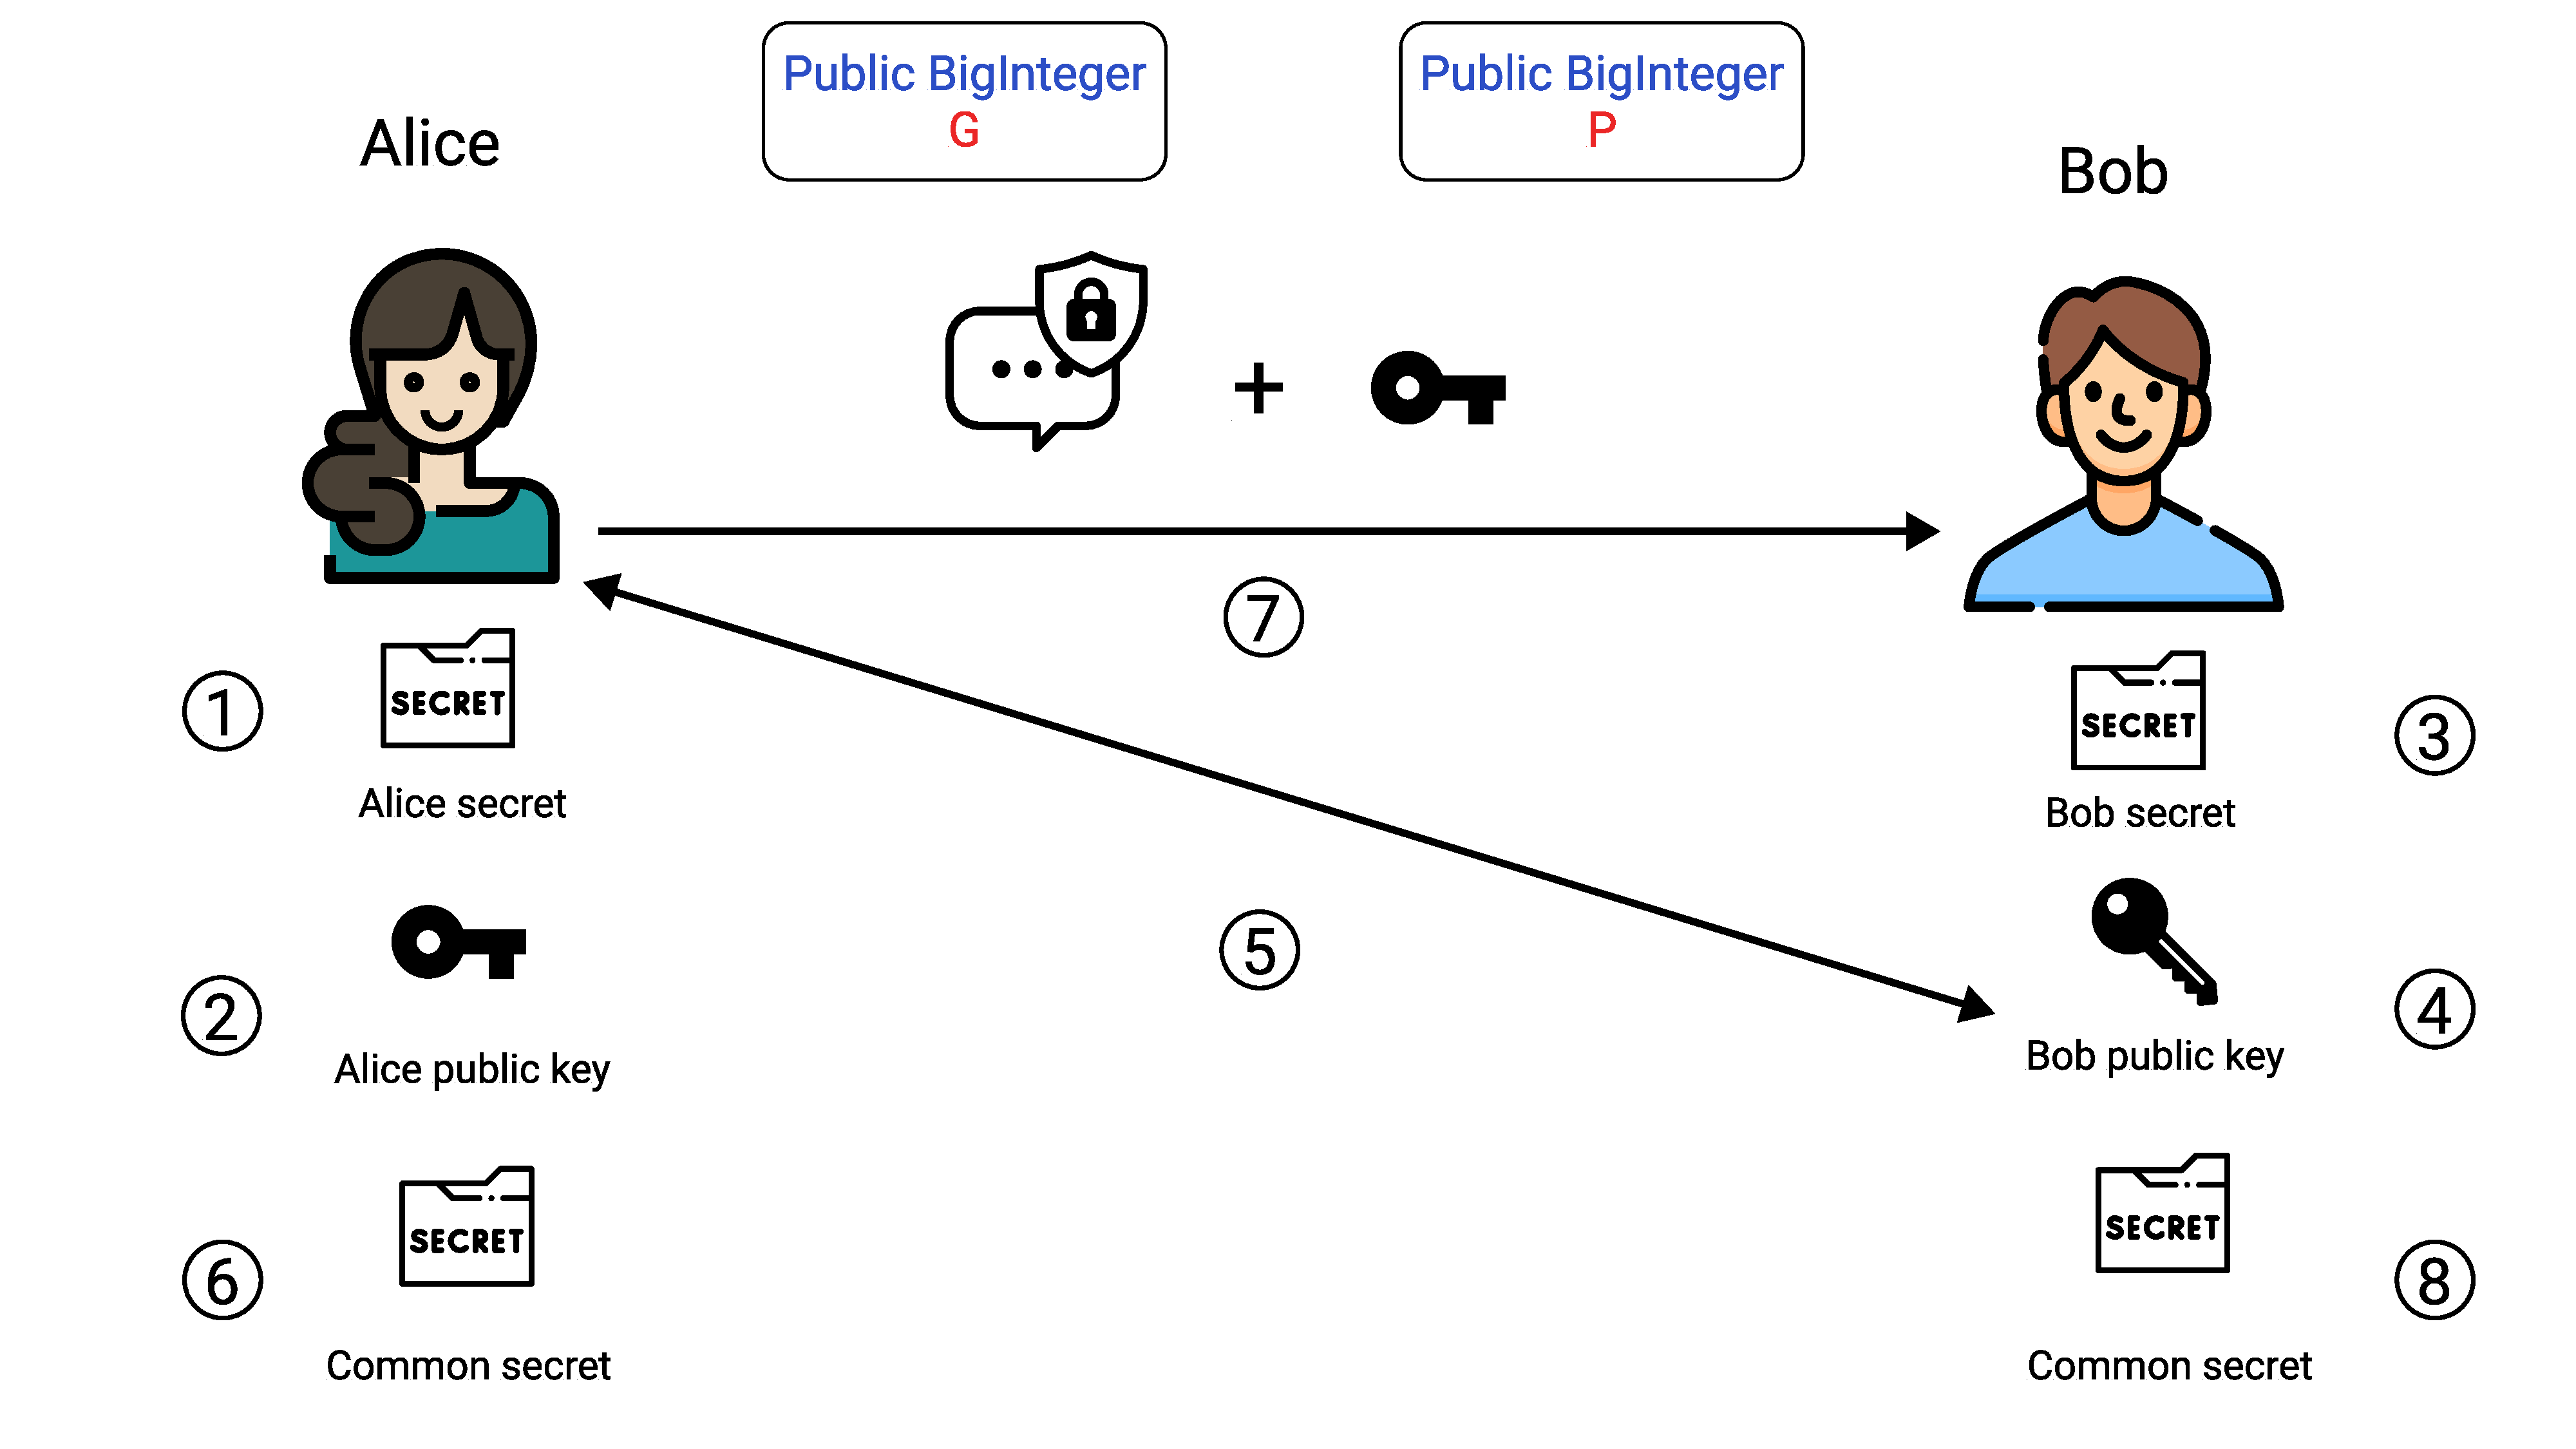
\includegraphics[width=1\textwidth]{Pictures/Key_Exchange}
    \caption{Secret chat encryption concept diagram. Source: }\label{fig:figure7}
\end{figure}
Assume that Alice wants to write a secret message to the Bob.
The secret chat encryption implemented as follows
\begin{enumerate}
    \item Given two public constants: $P, G$.
    \item Alice generates her secret $a$.
    \item Alice generates public key $A$ as $A=G^a \bmod P$ and shares it public.
    \item Bob generates his secret $b$.
    \item Bob generates public key $B$ as $B=G^b \bmod P$ and shares it public.
    \item Alice reads Bob's public key $B$.
    \item Alice calculates Common secret $s$ as $s = B^a \bmod P$.
    \item Alice encrypts message using AES256 algorithm, then sends it to Bob along her public key $A$.
    \item Bob calculates Common secret $s$ as $s = A^b \bmod P$ and decrypts message from Alice.
\end{enumerate}
Although, DH fits the key exchange concerns fine, the secret might be shared via RSA approach as well.
We discuss it in next section.